\documentclass[usenames,dvipsnames,acmsmall]{acmart}
\usepackage[utf8]{inputenc}
\usepackage[english]{babel}
\usepackage[nounderscore]{syntax}
\usepackage{bussproofs}
\usepackage{mathtools}
\usepackage[ruled,vlined,linesnumbered]{algorithm2e}
\usepackage{amsmath}
\usepackage{graphicx}
\usepackage{graphicx}
\usepackage{booktabs}
\usepackage{minted}
\usepackage{colortbl}
\usepackage{multirow}
\usepackage{minted}

\begin{document}
	\begin{figure}
		\begin{minted}{python}
	def count_heads(prob : float, n : int):
		x = 0
		while(n > 0):
			d = bernoulli.rvs(size=1, p=prob)[0]
			x = x + d
			n = n - 1
		return x
		\end{minted}
	\caption{Program to $count$ heads over $n$ bernoulli trials.}
	\end{figure}
	\begin{figure}
		\begin{minted}{python}
	if (prob <= 0.5) E(x) < 0.4 * n else E(x) >= 0.6 * n
		\end{minted}
	\caption{\texttt{Assert} we want to check for failure.}
	\end{figure}
	\begin{figure}
		\begin{minted}{python}
	
	double prob, path_prob = 1, choice_prob = 1;
	int sum = 0, n = 0;
	
	klee_make_symbolic(&prob, f"prob_sym_{i}");
	klee_make_symbolic(&n, f"n_symbolic");
	for i in range(n):
		int d;
		klee_make_symbolic(&d, f"d_sym_{i}");
	
		d = bernoulli(prob);
		(d == 1) ? choice_prob = prob : choice_prob = (1 - prob);
		path_prob = path_prob * choice_prob;
		
		sum = sum + d;
		
	klee_dump(path_prob)
	klee_dump(sum) // E[heads in "n" runs] 
		\end{minted}
		\caption{Program listing for $n$ bernoulli trails experiment with transformation for \texttt{KLEE}.}
	\end{figure}

We consider a independent $bernoulli$ trials here of flipping a fair coin "$n$" times. 
\[ 
{choice\_prob} = 
\begin{cases} 
	p & \textrm{if $d$ value is 1 corresponding to getting a "heads"} \\
	1-p & \textrm{if $d$ value is 0 corresponding to getting a "tails"}
\end{cases}
\]

concretely, on the $i^{th}$ run \texttt{$\vec{d}$} can have a value as below, \texttt{one-hot} encoded $w.r.t$ the outcome of $heads$ or $tails$.
\[
\vec{d}_{i} = encode(<0,0,0,1,1,0,1,1,1,0>)
\]

Based on the value of the $\vec{d}_{i}$, we get $w_{i}$ value using $choice\_prob$. 
\begin{equation}
	w_{i} = {(p)^{x_i} * (1-p)^{n-x_i}}
\end{equation}
where $x_i$ denotes the number of $heads$ in the $i^{th}$ randomized run and for $n$ runs. \texttt{n = 10} for the case in the above example. \\
\begin{equation}
	w_{i} = {(p)^{x_i} * (1-p)^{10-x_i}}
\end{equation}
We consider top "$k$" randomized runs now for the optimization query. The expression for \texttt{optimization} thus becomes 
\[	
	maximize(\sum_{i=1}^{k}{w_i})
\]
On substituting the value of $w_i$ from (1).
\begin{equation}	
	maximize(\sum_{i=1}^{k}{(p)^{x_i} * (1-p)^{n-x_i}})
\end{equation}

\begin{figure}
	\begin{equation}	
		Objective_1 = maximize(\sum_{i=1}^{k}{(p)^{x_i} * (1-p)^{n-x_i}}) \quad \mid \forall (i, j) \enspace [{x_i} \neq {x_j}]
	\end{equation}
	\caption{Optimization Expression for $k$ randomized paths}
	\label{eq:optimization-1}
\end{figure}

After performing the optimization above, we get different values of $\vec{d_i}$. For $i^{th}$ randomized run. we get a \texttt{single} one hot encoded \texttt{$\vec{d}$} vector. We show below the encoding for a few $i$ values. 
\[
\vec{d}_{1} = encode(<0,0,0,1,1,0,1,1,1,0>)
\]
\[
\vec{d}_{3} = encode(<0,1,0,1,1,0,0,0,1,0>)
\]
\[
\vec{d}_{4} = encode(<1,0,1,0,1,0,1,1,0,1>)
\]
\[
	....
\]
We run the optimization by renaming the $k$ \texttt{pse} variables set appropriately and then impose the $distinct$ clause so that we don't run the optimization on the same $randomized$ runs again. \\
\begin{equation}	
	\forall (i, j) \enspace [\vec{d_i} \neq \vec{d_j}]
\end{equation} \\
We approximate the value of $expected$ heads in the above program, with the following equations.
\begin{equation}	
	w_i = \prod_{j=1}^n choice\_prob_{i}(j) ,
	\quad
	sum_i = \sum_{j=1}^n components(\vec{d_i}) ,
\end{equation}
\begin{equation}
	EV(heads) = (\sum_{i=1}^{k}{w_i * sum_i}),
	\quad
	Error = n * prob - EV(heads)
\end{equation}
where both $w_i$ and $sum_i$ can both be computed from the corresponding $\vec{d_i}$ expression we get from the $model$  of the $optimization$ query Eq~\ref{eq:optimization-1}

For $k = 5$ \& $n = 10$ the two \texttt{constraint} sets and \texttt{optimization} expressions are as follows : 

\begin{equation}	
	w_1 = \prod_{j=1}^{10} choice\_prob_{1}(j) ,
	\quad
	sum_1 = \sum_{j=1}^{10} components(\vec{d_1}) ,
\end{equation}
\begin{equation}	
	w_2 = \prod_{j=1}^{10} choice\_prob_{2}(j) ,
	\quad
	sum_2 = \sum_{j=1}^{10} components(\vec{d_2}) ,
\end{equation}
\begin{equation}	
	w_3 = \prod_{j=1}^{10} choice\_prob_{3}(j) ,
	\quad
	sum_3 = \sum_{j=1}^{10} components(\vec{d_3}) ,
\end{equation}
\begin{equation}	
	w_4 = \prod_{j=1}^{10} choice\_prob_{4}(j) ,
	\quad
	sum_4 = \sum_{j=1}^{10} components(\vec{d_4}) ,
\end{equation}
\begin{equation}	
	w_5 = \prod_{j=1}^{10} choice\_prob_{5}(j) ,
	\quad
	sum_5 = \sum_{j=1}^{10} components(\vec{d_5}) ,
\end{equation}
\begin{equation}
	\vec{d_1} \neq \vec{d_2} \neq \vec{d_3} \neq \vec{d_4} \neq \vec{d_5}
\end{equation}
\begin{equation}
	EV(heads) = (\sum_{i=1}^{k}{w_i * sum_i}),
\end{equation}
\begin{equation}
	\enspace
	EV(heads) = (w_1 * sum_1 \enspace + \enspace w_2 * sum_2 \enspace + \enspace w_3 * sum_3 \enspace + \enspace w_4 * sum_4 \enspace + \enspace w_5 * sum_5)
\end{equation}
\begin{equation}
	\enspace
	Objective_2 = maximize(w_1 * sum_1 \enspace + \enspace w_2 * sum_2 \enspace + \enspace w_3 * sum_3 \enspace + \enspace w_4 * sum_4 \enspace + \enspace w_5 * sum_5)
\end{equation}
We can make multiple optimization $objectives$ be fulfilled in one query, but the best results are produced for the $Objective_2$ since it minimizes the $error$ most.

\begin{equation}
	Objective_{2} = maximize(\sum_{i=1}^{k}{w_i * x _i})
\end{equation}

\begin{figure}
	\centering
	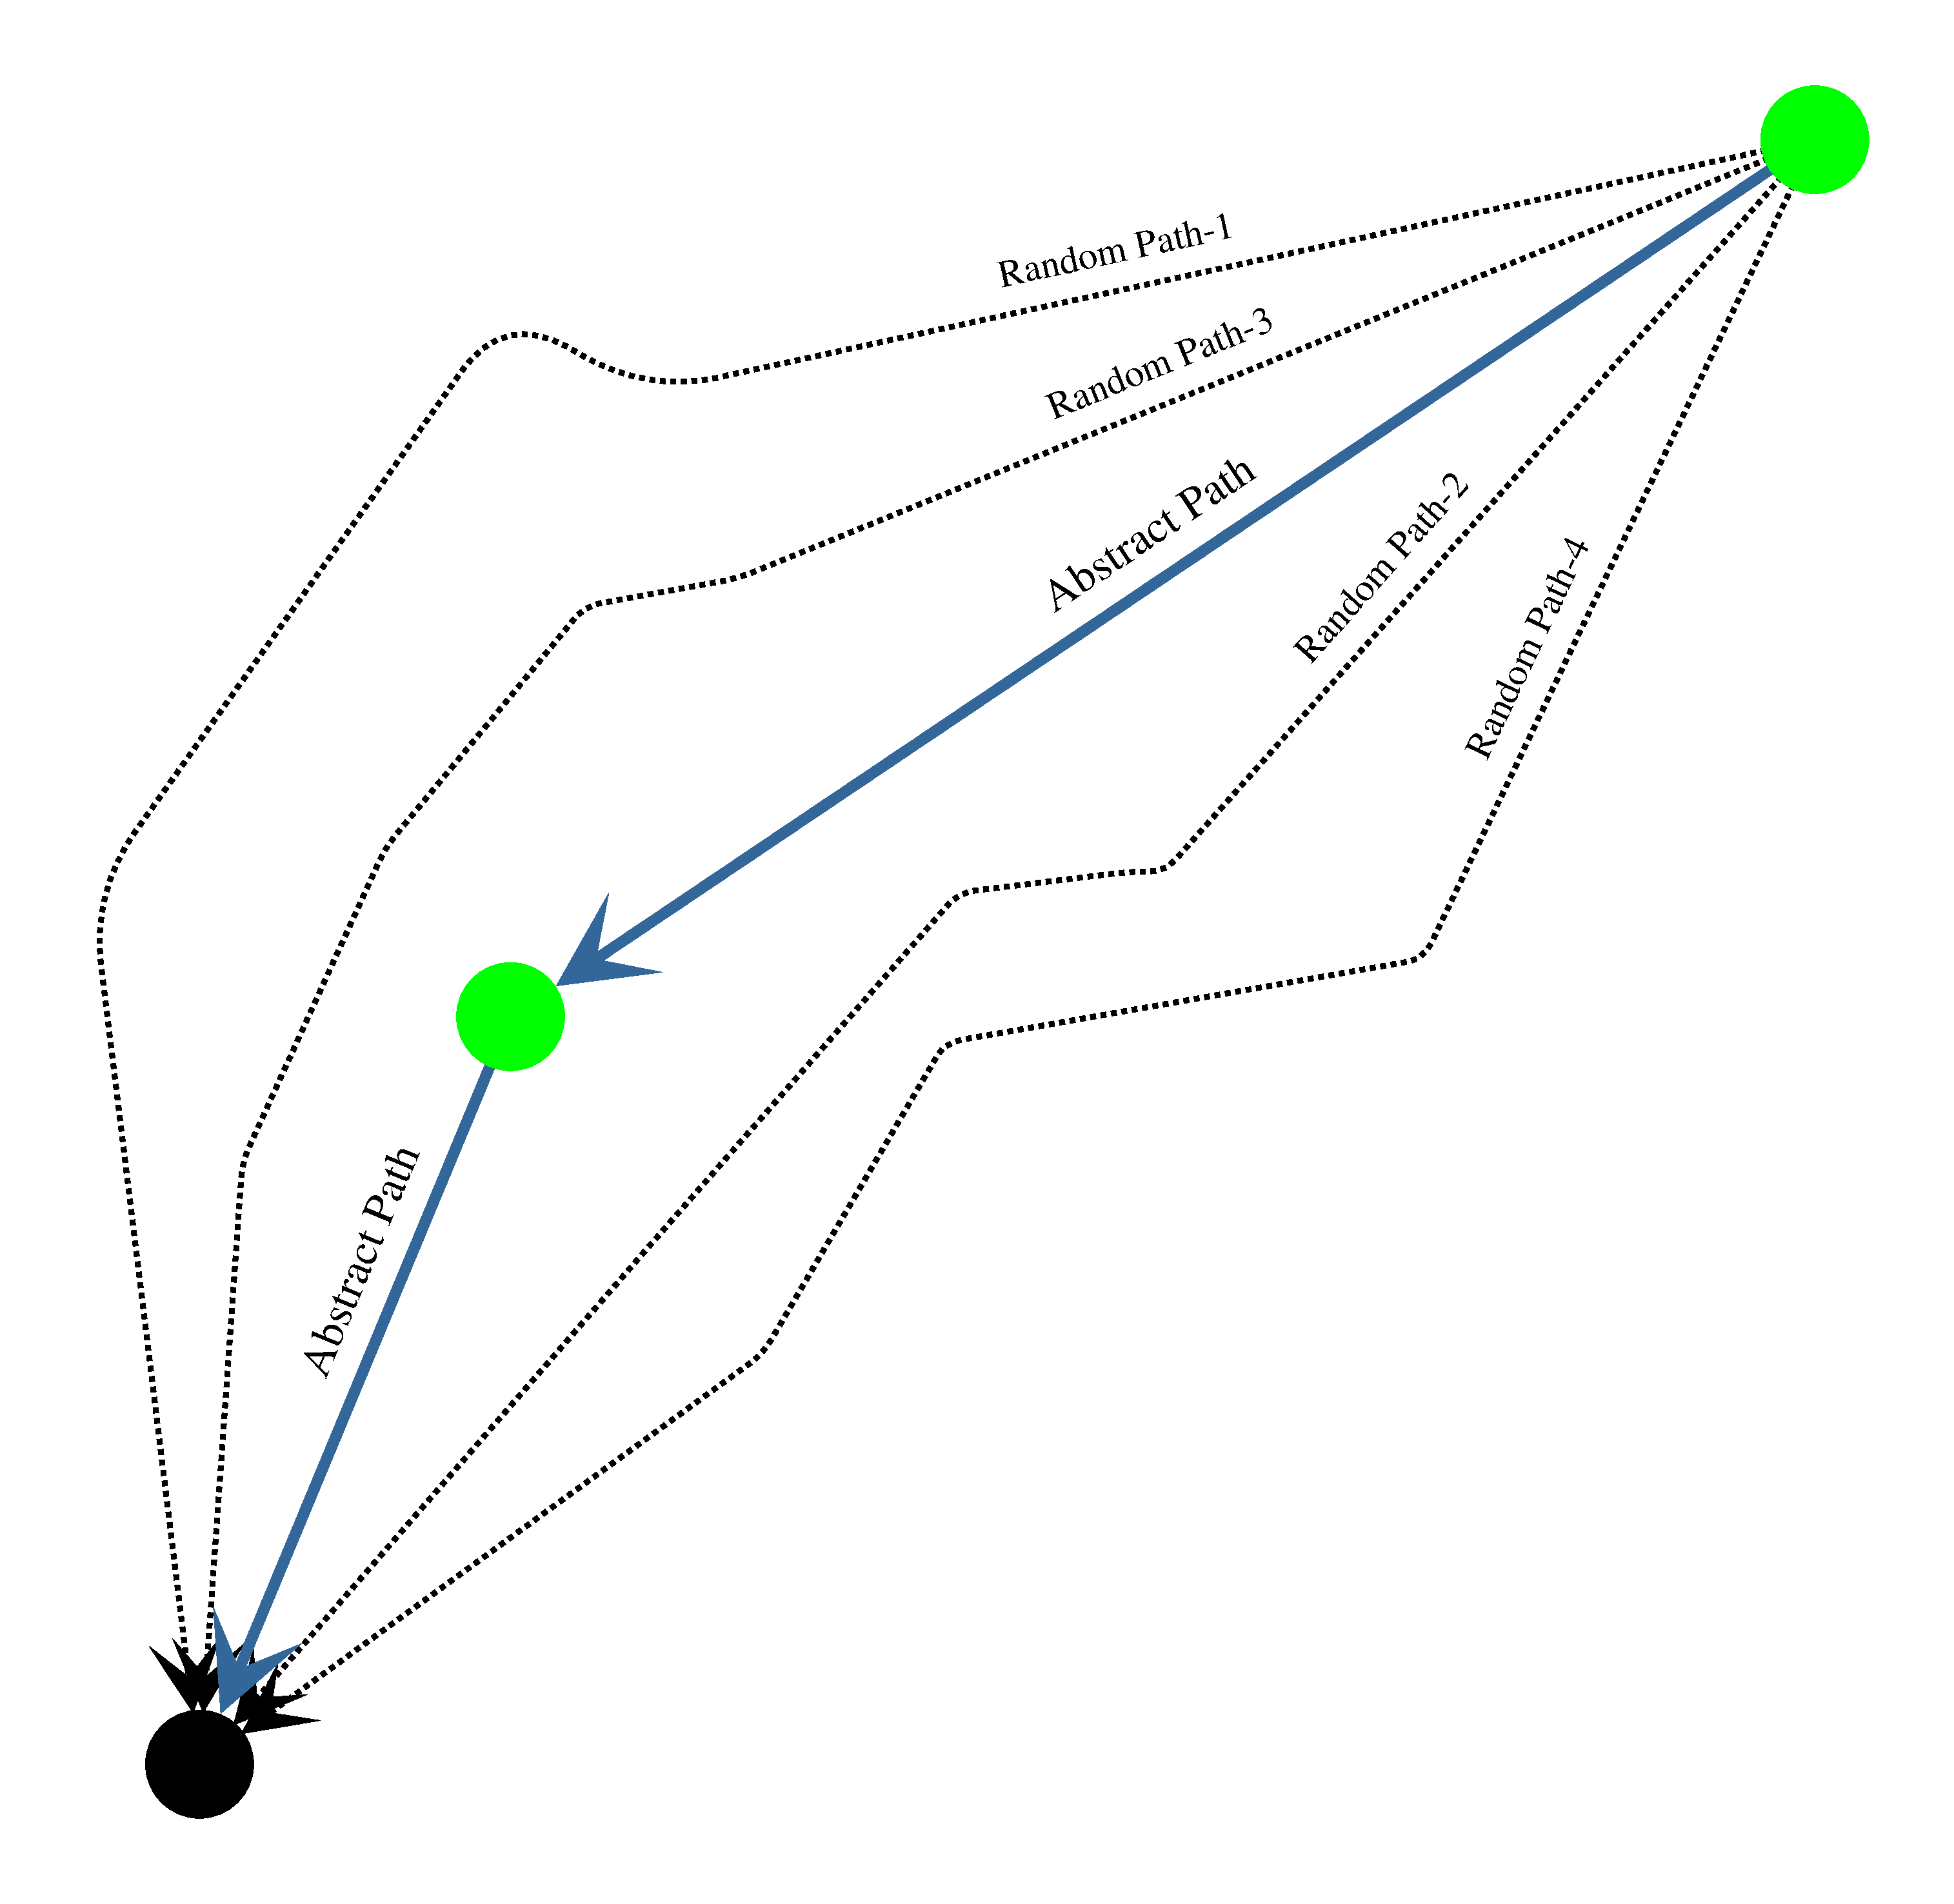
\includegraphics[scale=0.16]{abstract.pdf}
	\caption{Multiple $random$ paths corresponding to different $\vec{d}$'s but a single $abstract$ path.}
\end{figure}

\begin{figure}
	\begin{minted}{python}
	prob = 0.435, n = 8 (8 coin flips), k = 240 (randomized paths)
	prob = 0.551, n = 5 (5 coin flips), k = 27 (randomized paths) 
	\end{minted}
	\caption{Values for \texttt{Assert} failure.}
\end{figure}


\end{document} 